\section{Kopplingsschema}
Robotens elektronik är uppdelad på två virkort. Därför presenteras här ett kopplingsschema för varje virkort.

\subsection{Sensorenhet}

\nyBild{kopplingsschema_sensor.png}{Kopplingsschema för virkortet som innehåller sensorenheten.}{senskoppling}{1}

\subsection{Kommunikationsenhet, Armenhet, Chassienhet}
\begin{figure}[H]
\centering
 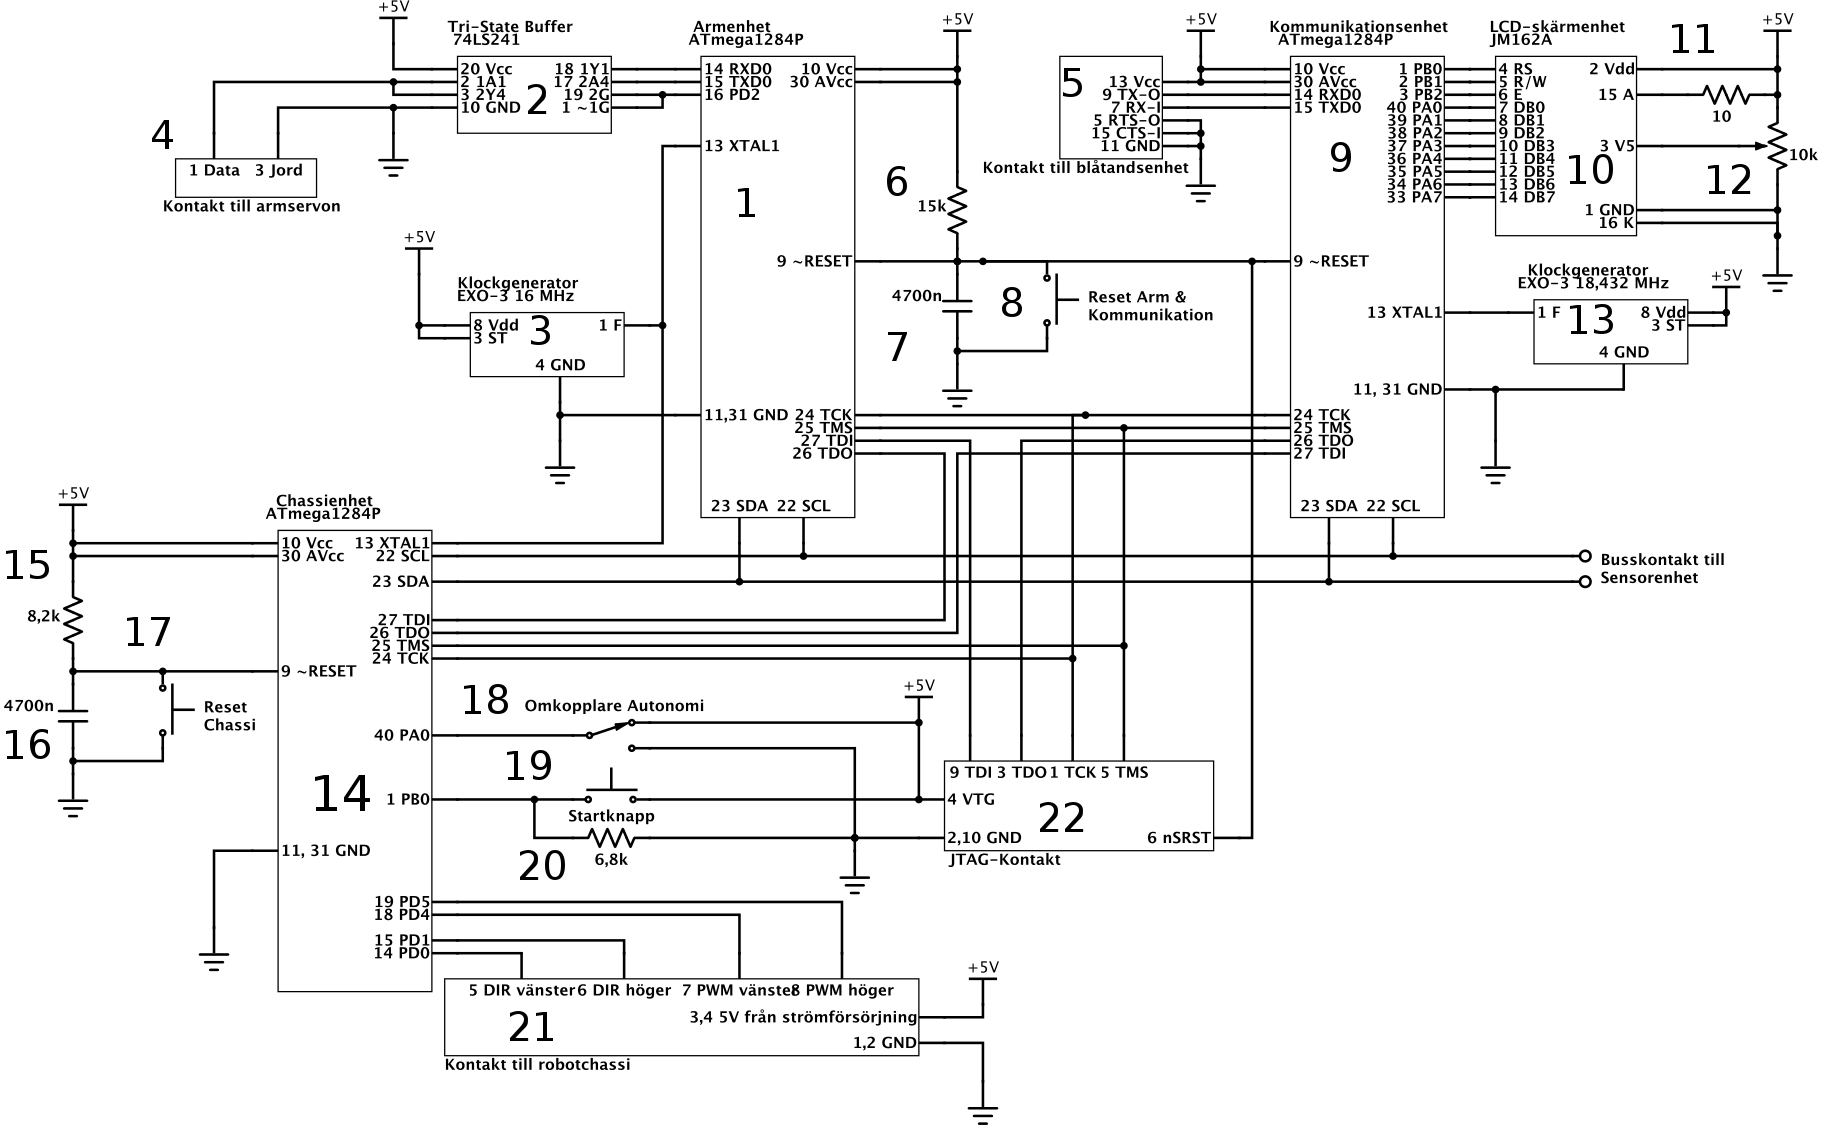
\includegraphics[angle=90,width=0.85\textwidth]{bilder/chassiarmkomm.png}
  \emph{\caption{Kopplingsschema över virkortet som innehåller kommunikationsenheten, chassienheten och armenheten.} \label{fig:chassiarmkomm}}
  
\end{figure}

\textbf{Komponentförteckning}
\begin{packed_enumerate}
\item[1.] Processor Armenhet, ATmega 1284P
\item[2.] Tri-state buffer, 74LS241
\item[3.] Klockgenerator för Armenhet och Chassienhet, EXO-3 16 MHz  
\item[4.] Kontakt för kabel till armservon
\item[5.] Kontakt för kabel till blåtandsenhet
\item[6.] Pullup-resistor för reset av Kommunikationsenhet och Armenhet, 15 k$\Omega$
\item[7.] Kondensator för reset av Kommunikationsenhet och Armenhet, 4700 nF
\item[8.] Resetknapp för Kommunikationsenhet och Armenhet
\item[9.] Processor Kommunikationsenhet, ATmega 1284P
\item[10.] Skärmenhet för LCD-skärm, JM162A
\item[11.] Resistor för att begränsa strömmen till LCD-skärmens bakgrundsbelysning, 10 $\Omega$
\item[12.] Potentiometer för att justera LCD-skärmens kontrast, 0 - 10 k$\Omega$
\item[13.] Klockgenerator för Kommunikationsenhet, EXO-3 18.432 MHz
\item[14.] Processor för Chassienhet, ATmega 1284P
\item[15.] Pullup-resistor för reset av Chassienhet, 8,2 k$\Omega$
\item[16.] Kondensator fö reset av Chassienhet, 4700 nF
\item[17.] Resetknapp för Chassienhet
\item[18.] Omkopplare för att växla mellan autonomt och fjärrstyrt läge
\item[19.] Startknapp för att påbörja autonom drift
\item[20.] Pulldown-resistor för startknappen
\item[21.] Kontakt för kabel till robotchassi, tillför spänning +5 V till virkortet
\item[22.] Kontakt för JTAG-kabel.
\end{packed_enumerate}


\section{Utdrag från programlistning}
\emph{(ca 5-10 sidor så att vi kan bedöma kodens läsbarhet mm.) och eventuell VHDL-kod}
\section{Övriga bilagor?}
